\documentclass[10pt,conference]{IEEEtran}
\usepackage{amsmath,amssymb}
\usepackage{booktabs}
\usepackage{graphicx}
\usepackage{url}
\usepackage{xcolor}
\pdfmapfile{+cm.map}

\title{A Safety-Gated Chaos-Metric Supervisor for UAVs in
Lorenz-Derived Disturbances}

\author{\IEEEauthorblockN{UAV Chaos Supervisor Research Workstream}
\IEEEauthorblockA{Reproducible software and simulation study}}

\begin{document}
\maketitle

\begin{abstract}
Small unmanned aerial vehicles can experience rapidly varying disturbances for
which a conventional threshold on a single sensor is an incomplete supervisory
signal. This work presents a reproducible software architecture that converts
inertial telemetry into a bounded instability indicator and uses it to select
conservative, high-level flight strategies. The implementation combines a
Lorenz-system disturbance generator, a rolling acceleration/jerk metric, a
Rosenstein-style largest-Lyapunov estimator for offline analysis, a strict
structured-proposal boundary for optional language-model assistance, and a
simulation-gated PX4 setpoint adapter. A matched-seed 35-s reference experiment
reduced horizontal RMS error from 72.21 m to 21.84 m and maximum error from
99.97 m to 29.43 m when supervision was enabled. These values validate the
dataflow, decision gates, reproducibility, and reporting pipeline; they are not
evidence of aircraft-level stability or of chaos in a physical flight. The
paper documents the complete design, implementation, results, and limitations
of the project in a form suitable for repeatable extension to PX4/Gazebo.
\end{abstract}

\begin{IEEEkeywords}
UAV supervision, chaos metric, Lyapunov exponent, PX4, ROS 2, safety gate,
Lorenz system
\end{IEEEkeywords}

\section{Introduction}
Autonomous UAVs must remain controllable while their state estimates and
external disturbances change faster than a human operator can react. The
project reported here investigates a narrow supervisory layer rather than a
replacement flight controller: measured acceleration is summarized as an
instability signal, and a policy selects a bounded intent such as holding,
reducing speed, or returning home. The central engineering requirement is that
an uncertain metric or optional remote model must never directly issue motor
commands.

The implementation has two complementary uses. First, a deterministic offline
backend makes the complete loop testable without a running ROS graph or
hardware. Second, ROS 2 nodes define the same metric and decision boundaries
for PX4 SITL and Gazebo. The distinction matters: the offline backend is a
surrogate for integration testing, not a rigid-body flight model. This paper
therefore reports quantitative surrogate results and separately describes the
live deployment path and its safety restrictions.

\section{System Design}
Figure~\ref{fig:results} shows the outputs generated by the reference pipeline.
The software is organized into four boundaries: (i) disturbance and telemetry,
(ii) metric estimation, (iii) strategy selection, and (iv) bounded execution.
The recorder subscribes to PX4 \texttt{/fmu/out/vehicle\_odometry} and
\texttt{/fmu/out/sensor\_combined} using best-effort QoS and stores timestamped
CSV files. The path viewer is intentionally observational: it plots local-NED
horizontal motion (north/east) and issues no vehicle command.

The live metric node maintains up to 1200 scalar accelerometer samples. After
300 samples it publishes JSON on \texttt{/uav/chaos\_metric}, including a
timestamp, bounded instability, Lyapunov estimate, sample count, and quality.
The optional ROS boundary publishes a validated high-level command on
\texttt{/uav/supervisor/command}. The direct PX4 adapter consumes the metric and
odometry, publishes bounded position setpoints, and is enabled only when
\texttt{UAV\_SIMULATION=1}; optional offboard/arming commands require an
additional command-line flag.

\subsection{Disturbance and reference backend}
The disturbance generator integrates the Lorenz equations\cite{lorenz}
\begin{equation}
 \dot{x}=\sigma(y-x),\quad \dot{y}=x(\rho-z)-y,\quad
 \dot{z}=xy-\beta z,
 \label{eq:lorenz}
\end{equation}
with $(\sigma,\rho,\beta)=(10,28,8/3)$. The state is scaled by
$s_w=0.12$ to obtain three disturbance components. In the reference backend,
position and velocity are advanced with a fixed $\Delta t=0.02$ s Euler step;
the disturbance is added to a damped acceleration model and small seeded
Gaussian noise. The vertical command tracks 5 m. The baseline always holds its
strategy; the supervised case calls the supervisory agent at most once per
second.

\subsection{Instability metrics}
The causal rolling metric used by the reference loop is computed over the most
recent 160 samples. For acceleration samples $a_k$, it combines mean energy and
jerk roughness:
\begin{equation}
 \begin{aligned}
 I_k&=1-\exp\bigl(-0.018\,\overline{\|a\|}_k
 -0.0015\,\overline{\|\Delta a/\Delta t\|}_k\bigr),\\
 &\qquad 0\leq I_k<1.
 \end{aligned}
 \label{eq:indicator}
\end{equation}
This signal is deliberately an instability indicator, not a classifier that
proves a UAV trajectory is chaotic. For offline analysis, the package also
implements a Rosenstein-style estimate following Rosenstein et al.~\cite{rosenstein}.
A scalar uniformly sampled signal is
delay embedded with dimension $m$ and delay $\tau$; temporally separated nearest
neighbors are found with a Theiler window, and a linear fit to mean log-distance
growth gives
\begin{equation}
 \hat{\lambda}_{\max}=\operatorname{slope}_t\left[
 \left\langle\log d_i(t)\right\rangle_i\right].
 \label{eq:lyap}
\end{equation}
Timestamp intervals are inferred from the median positive interval and the
estimator rejects strongly irregular sampling. This guard is important for
telemetry because a positive finite-window estimate can result from noise,
forcing, or sampling artifacts.

\subsection{Safety-gated supervision}
The allowed strategy set is $\{\texttt{hold},\texttt{reduce\_speed},
\texttt{return\_to\_home}\}$. Observations contain instability, horizontal
position error, altitude, timestamp, and vehicle availability. The deterministic
policy first rejects unavailable, non-finite, future, or stale state (older than
1 s). It then applies a low-altitude hold gate below 1 m, requests return home
when position error exceeds 8 m, requests reduced speed when $I>0.15$, and
otherwise holds. Structured remote proposals must contain exactly
\texttt{strategy} and \texttt{timestamp\_s}; the same freshness, availability,
altitude, and threshold checks are applied after parsing. Any failed proposal
falls back to deterministic hold/policy behavior.

The optional agent tries an OpenAI-compatible endpoint, then Gemini, and then
the deterministic policy. Temperature is zero and a function schema constrains
the remote response. Neither provider is required for the reference results:
the stored runs used the deterministic fallback because no credentials were
needed. The separation prevents a network response from bypassing local safety
logic and makes experiments reproducible.

\section{Experimental Method}
The reference experiment was run with duration 35 s, $\Delta t=0.02$ s, wind
scale 0.12, target altitude 5 m, and seed 7. Baseline and supervised runs used
identical initial conditions and the same Lorenz sequence. Each run generated
1750 samples, timestamped telemetry CSV, and JSON metadata containing the
configuration, summary, action events, and backend label. Evaluation used
horizontal error $e_k=\sqrt{x_k^2+y_k^2}$, its RMS, its maximum, and altitude
mean/standard deviation. The comparison is intentionally matched, but it is
not a statistical study: it is one deterministic seed used to exercise the
integration boundary.

\begin{table}[t]
\centering
\caption{Matched-seed deterministic reference results (35 s, seed 7).}
\label{tab:results}
\footnotesize
\begin{tabular}{lrrr}
\toprule
Metric & Baseline & Supervised & Change\\
\midrule
Horizontal RMS (m) & 72.206 & 21.839 & $-69.8\%$\\
Horizontal maximum (m) & 99.972 & 29.432 & $-70.6\%$\\
Peak instability & 0.0895 & 0.0895 & 0\\
Mean instability & 0.0699 & 0.0699 & 0\\
Mean altitude (m) & 8.605 & 8.701 & $+1.1\%$\\
Altitude std. (m) & 2.837 & 2.216 & $-21.9\%$\\
\bottomrule
\end{tabular}
\end{table}

\section{Results}
Table~\ref{tab:results} shows a substantial reduction in horizontal error for
the supervised reference trajectory while the disturbance and metric traces
remain identical. The supervised run changed from \texttt{hold} to
\texttt{return\_to\_home} at 4.78 s; the baseline had no action events. The
identical peak and mean instability confirm that the comparison changes the
response policy rather than the disturbance. The altitude statistics also show
that the reduced horizontal error was not obtained by removing the vertical
state from the simulation.

\begin{figure}[t]
\centering
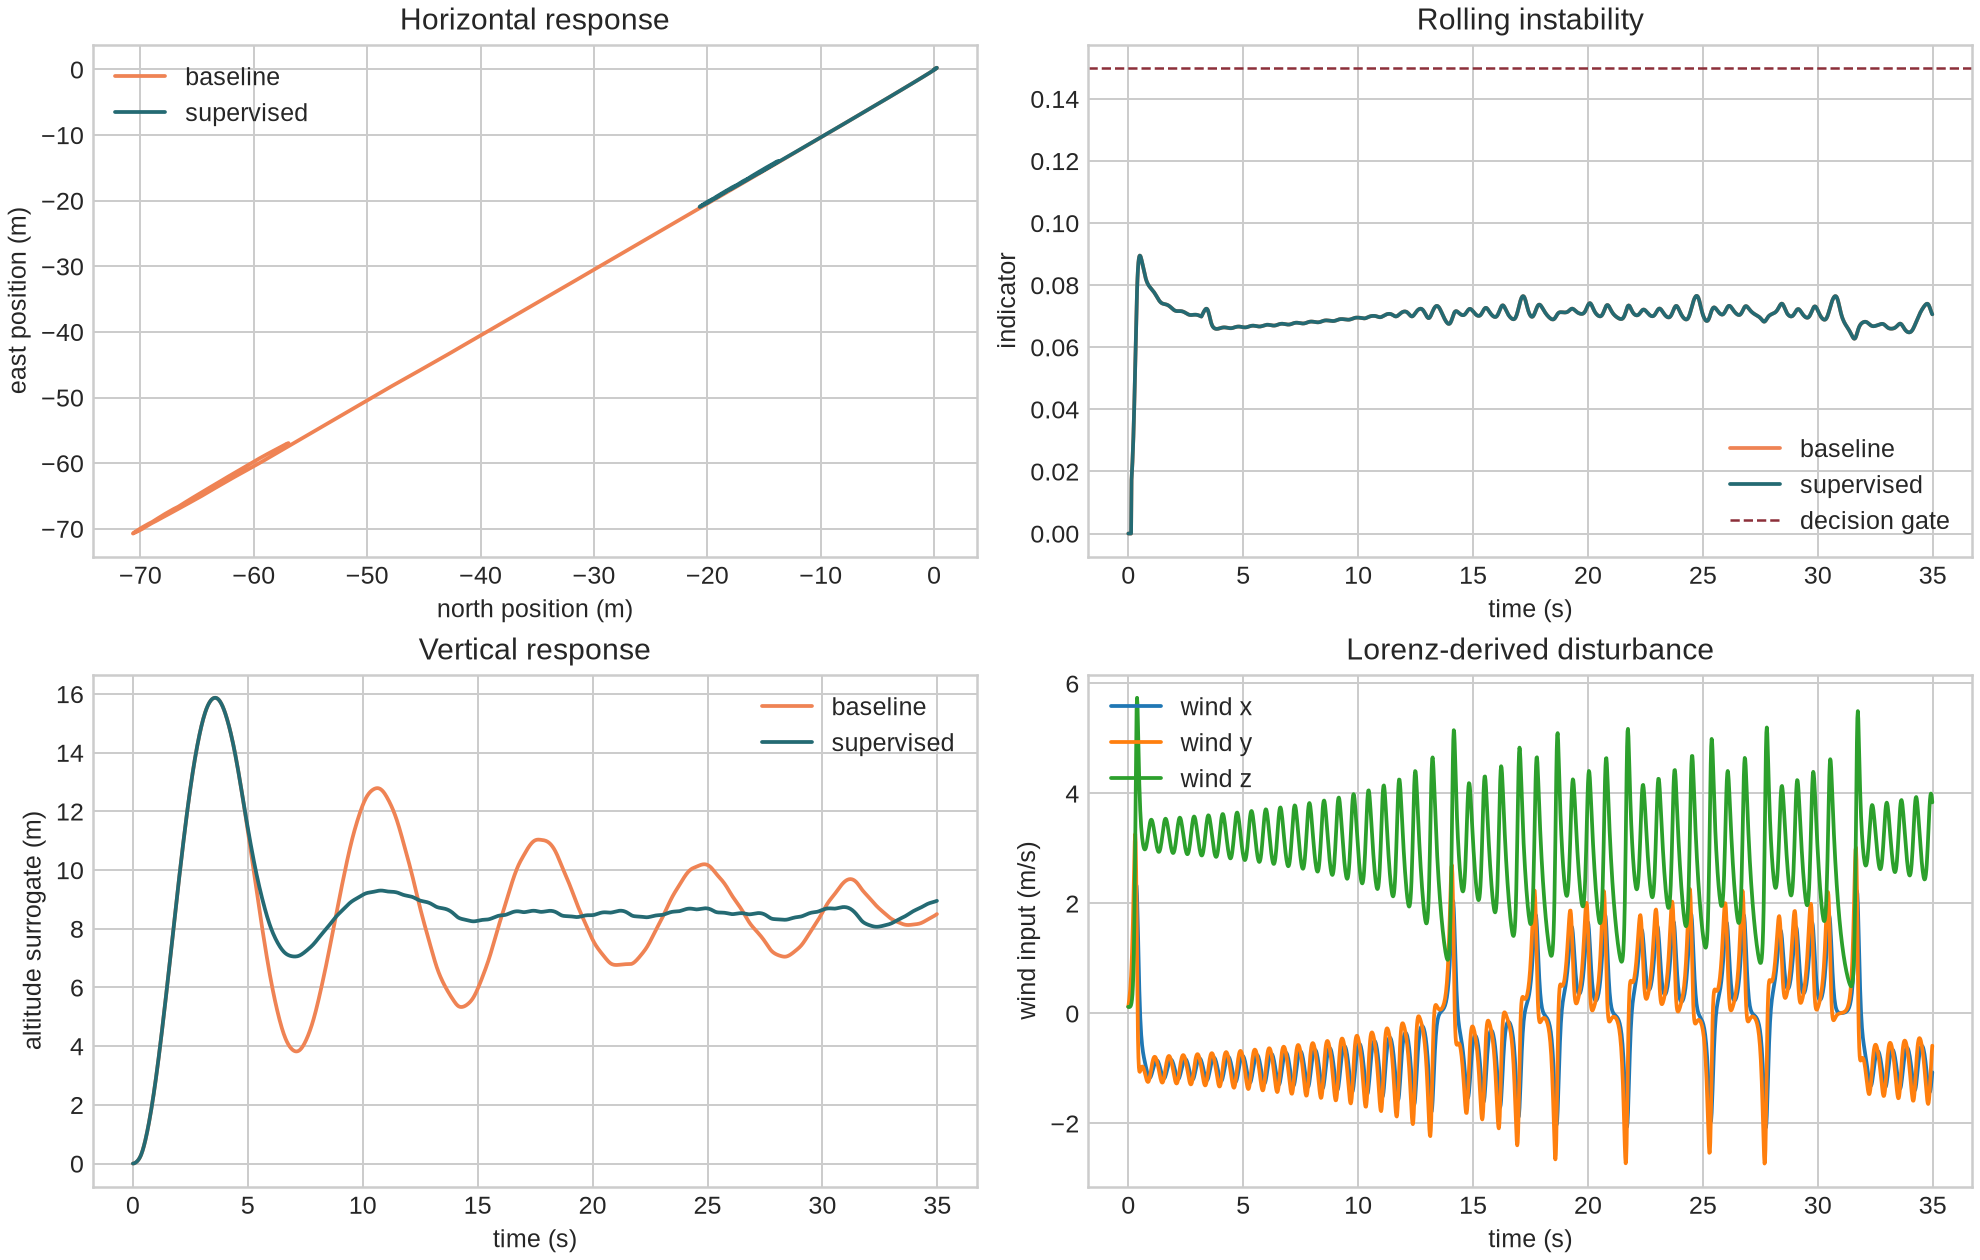
\includegraphics[width=\columnwidth]{integration_results.png}
\caption{Reference integration output: baseline/supervised trajectory,
instability, altitude, and Lorenz-derived wind. This figure is a surrogate
validation artifact, not a flight-test plot.}
\label{fig:results}
\end{figure}

The result demonstrates that the end-to-end artifacts are connected: Lorenz
integration produces the disturbance, telemetry records the state, the metric
is available to the decision loop, a safety-gated strategy changes the bounded
reference dynamics, and the report generator consumes the resulting CSV/JSON
files. It does not establish that the metric is predictive of real UAV
instability, that return-to-home is optimal, or that an LLM improves safety.

\section{Implementation and Reproducibility}
The package is a ROS 2 Python package with NumPy and SciPy for numerical work;
PX4 message types are imported only by live ROS nodes. From the project root,
the reference experiment and paper artifacts can be reproduced with:
\begin{verbatim}
PYTHONPATH=ros2_ws/src/telemetry_node \\
python3 -m \\
  telemetry_node.experiment_cli \\
  demo \\
  --duration 35 --seed 7 \\
  --output-dir results/demo
PYTHONPATH=ros2_ws/src/telemetry_node \\
python3 -m \\
  telemetry_node.experiment_cli \\
  report \\
  results/demo/baseline_telemetry.csv \\
  results/demo/supervised_telemetry.csv \\
  --output-dir results/report
\end{verbatim}
The repository also contains unit/integration tests for the research pipeline,
the runbook for building Micro-XRCE-DDS-Agent, PX4 SITL, ROS 2, and the
headless live launcher, following the PX4 ROS 2 integration model~\cite{px4}.
Live use requires verification that the Gazebo plugin
actually consumes the generated wind and that applied forces are observed in
telemetry; generating a wind CSV alone is not such verification.

\section{Limitations and Future Work}
The main limitation is model fidelity. The reported backend is a deterministic
surrogate with a simple damped point-mass update, not PX4 control allocation,
vehicle dynamics, aerodynamic drag, sensor delay, estimator error, or a
validated Gazebo force model. The single matched seed also prevents claims
about statistical significance. Future evaluation should use multiple seeds,
matched disturbances, sensitivity sweeps over embedding and metric parameters,
and flight-level metrics such as settling time, control effort, collision
margin, and failsafe behavior.

The live estimator must be evaluated against known disturbances and controlled
telemetry loss. The current quality score accounts for sample count and timing
irregularity, but a production system should add explicit confidence thresholds
and a tested loss-of-data behavior. Before any physical deployment, the bounded
setpoint adapter needs independent review of NED/FRD frames, arming state,
offboard transitions, geofencing, watchdog behavior, and manual override. The
language-model path should remain advisory and fail closed; deterministic
policies and formal interface validation are the safety authority.

\section{Conclusion}
This project provides a compact, reproducible supervisory architecture for
studying disturbance-aware UAV behavior. Its strongest result is not a claim of
chaos-induced flight improvement, but a traceable engineering boundary: an
interpretable bounded metric feeds a strict policy, optional remote proposals
are validated locally, and actuation is simulation-gated. In the stored
reference experiment, this loop reduced horizontal RMS and maximum error by
approximately 70\% under identical Lorenz forcing. The next scientifically
necessary step is validated PX4/Gazebo experimentation, followed by systematic
uncertainty and safety evaluation before any real vehicle use.

\begin{thebibliography}{00}
\bibitem{lorenz} E. N. Lorenz, ``Deterministic nonperiodic flow,''
  \emph{J. Atmospheric Sciences}, vol. 20, no. 2, pp. 130--141, 1963.
\bibitem{rosenstein} M. T. Rosenstein, J. J. Collins, and C. J. De Luca,
  ``A practical method for calculating largest Lyapunov exponents from small
  data sets,'' \emph{Physica D}, vol. 65, pp. 117--134, 1993.
\bibitem{px4} PX4 Development Team, ``PX4 User Guide: ROS 2 User Guide,''
  PX4 Autopilot documentation, accessed Nov. 2026. [Online]. Available:
  \url{https://docs.px4.io/main/en/ros/}
\bibitem{repo} UAV Chaos Supervisor Research Workstream, ``UAV chaos
  supervisor v2,'' source repository, 2026.
\end{thebibliography}

\end{document}
